\usetikzlibrary{math}

\newcommand{\barwidth}{.5cm}

\newcommand{\drawaxes}[1]{
  \draw [->] (-.2, 0) -> (4 * \barwidth + .2cm, 0) node[anchor=west] {$x$};
  \draw [->] (-.2, 0) -> (-.2, 5.2) node[anchor=south] {$#1$};
  \foreach \x in {0, ..., 4}
    \draw (\x * \barwidth, -1pt) -- (\x * \barwidth, 1pt);
  \foreach \x/\char in {0.5/$a$, 1.5/$b$, 2.5/$c$, 3.5/$d$}
    \draw (\x * \barwidth, 0) node[anchor=north, text height=8] {\char};
}

\newcommand{\drawbar}[3]{
  \draw[#3] (#1, 0) -- (#1, 12.5cm * #2) -- (\barwidth + #1, 12.5cm * #2) --
  (\barwidth + #1, 0);
}

\newcommand{\drawpmf}{
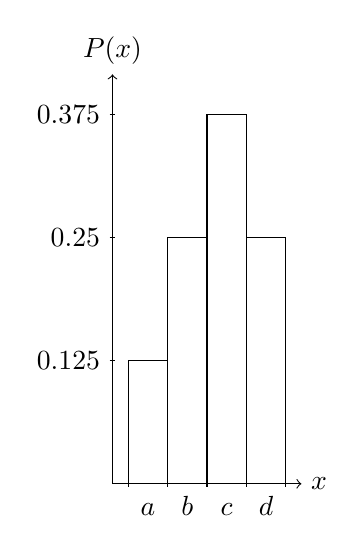
\begin{tikzpicture}
  \drawaxes{P(x)}
  \foreach \y in {0.125, 0.25, 0.375}
    \draw (-.2cm - 1pt, 12.5 * \y) node[anchor=east] {$\y$}
      --  (-.2cm + 1pt, 12.5 * \y);
  \drawbar{0 * \barwidth}{0.125}{};
  \drawbar{1 * \barwidth}{0.25 }{};
  \drawbar{2 * \barwidth}{0.375}{};
  \drawbar{3 * \barwidth}{0.25 }{};
\end{tikzpicture}
}

\newcommand{\drawapprox}[2]{
\begin{tikzpicture}
  \tikzmath{
    \splus = #1 + 1;
    \yunit = 12.5 / \splus;
  }
  \draw[xstep=\barwidth, ystep=\yunit, lightgray, very thin]
    (0, 0) grid (4 * \barwidth, 5.2);
    \drawaxes{s'}
  \foreach \y [parse=true, count=\s] in {\yunit, 2 * \yunit, ..., 5.2}{
    \node (tick) at (-.2cm, \y) {};
    \draw ($(tick) - (1pt, 0)$) -- ($(tick) + (1pt, 0)$);
    \draw ($(tick) - (0, \yunit / 2) - (.05, 0)$) node[anchor=east]
      {\pgfmathparse{int(\s - 1)} #2 $\pgfmathresult$};
  }
  \foreach \x/\freq/\start in {0/1/0, 1/2/1, 2/3/3, 3/2/6}{
    \foreach \y [parse=true, count=\s] in {\yunit, 2 * \yunit, ..., 5.2}{
      \tikzmath{
        \snew = int(8 * int((\s - 1) / \freq) + mod((\s - 1), \freq) + \start);
        if \snew>#1 then {\toprint = \snew;} else {let \toprint = ;};
        }
      \draw ($6.25/\splus*(0, -1) + 0.45*(\barwidth,0)
      + \s*(0, 12.5 / \splus) + \x*(\barwidth, 0)$) node [text=lightgray] {#2 $\toprint$};
    }
  }
  \drawbar{0 * \barwidth}{0.125}{thin, gray};
  \drawbar{1 * \barwidth}{0.25} {thin, gray};
  \drawbar{2 * \barwidth}{0.375}{thin, gray};
  \drawbar{3 * \barwidth}{0.25} {thin, gray};
  \foreach \x/\freq/\start in {0/1/0, 1/2/1, 2/3/3, 3/2/6}{
    \foreach \y [parse=true, count=\s] in {\yunit, 2 * \yunit, ..., 5.2}{
      \tikzmath{
        \snew = int(8 * int((\s - 1) / \freq) + mod((\s - 1), \freq) + \start);
        if \snew<=#1 then {\toprint = \snew;} else {let \toprint = ;};
        }
      \draw ($(0, -\yunit / 2) + 0.47*(\barwidth,0)
      + \s*(0, \yunit) + \x*(\barwidth, 0)$) node {#2 $\mathbf\toprint$};
    }
  }
\end{tikzpicture}
}

\newcommand{\intervalwidth}{0.8\textwidth}
\newcommand{\drawinterval}{
\begin{tikzpicture}
  \draw (0, 0) -- (\intervalwidth, 0);
  \draw (0, 0) -- (0, 4pt) node [anchor=south] {$0$};
  \draw (\intervalwidth, 0) -- (\intervalwidth, 4pt) node [anchor=south] {$1$};
\end{tikzpicture}
}
